    \documentclass[12pt]{article}
    \usepackage{amsmath}
    \usepackage{graphicx}
    \usepackage{multirow}
    \usepackage{booktabs}
    \usepackage{subfigure}
    \usepackage{verbatim}
    \usepackage{color}
    \usepackage{hyperref}
    \usepackage{url}
    \usepackage{axessibility} 
    \usepackage{soul}
    
    
    \begin{document}

    \title{Phys 132 -- Worksheet 3 -- 30868664}
    \author{Samuel Hedges}
    \date{\today}
    \maketitle
    
\section{Abstract}
    \subsection{Original Abstract}
 In this experiment the Photoelectric effect is studied experimentally to find the work function of silver oxide when high energy photons are incident upon its surface. The results of this experiment will show the theory behind Einstein’s 1921 Noble prize \cite{1921 Nobel} can be proved experimentally and is an example of the particle nature of light. This experiment will also attempt to measure the ratio Planck’s constant to the standard charge of the electron to find if their values match the theory, both of which are key parts in our understanding of the nature of quantum physics.\\

    \subsection{Improved Abstract}
The Photoelectric effect is a critical part of the field of quantum physics whereby an electron is emitted by a metal surface when a high energy light is shone (incident) upon the surface. The photoelectric effect was first observed by Henrik Hertz in 1887 \cite{Hertz}. In this report I  investigate the value of the Planck's constant, [h], and the work function [$\phi$]. This will be achieved through a set up where a mercury light source is incident upon a silver oxide anode. a stopping voltage was measured and from this and with knowledge of the charge of the electron I was able to calculate the value for h \& $\phi$ constants, and compare them to given values. In my experiment I was able to conclude that both the values of h and $\phi$ were correct, strongly agreeing with the experiment with a high level of accuracy. This result more generally show that the model of quantum physics is able to correct predict the outcome of the experiment and give us accurate values for constants and therefore the model can be adopted and tested against other problems in the quantum field like electrodynamics.\\

\textit{The reason I have included more of a preamble that wasn't in the original is to try to help/explain to non-specialists about the photoelectric effect. In this Abstract I have also included more explanation about what the experiment's results and what it was trying to measure as it help prospect readers to understand what I am trying to achieve from the outset and may make them more interested in reading the paper as a whole. I have also grounded the experiment in the field of quantum physics which is something that I missed in the original and may also help to entice prospect readers along with the added bonus of being able to show how the physics fits in the broader field}

\section {Introduction}
\subsection{Original Introduction }
 The study of particles at the quantum level gives rise to new theories which can be used to innovate
technology to be more compact and more powerful. One of the most important theories is the photoelectric effect, as this phenomenon can give insight into how light can act as both a wave and a
particle (wave particle duality). The study of the photoelectric effect was one of the first insights into the nature of quantum physics. By studying this simple phenomenon, we get an insight into the probabilistic nature of quantum physics.\\

The photoelectric effect is employed in many antiquated and modern technologies such as oscilloscopes, cathode ray television screens, fluorescent lighting and can even be used for chemical analysis. Therefore, understanding and fulfilling successful experiments based on the theory is critical to our understanding of the universe at large.\\

Our understanding today of the photoelectric effect primarily comes from Albert Einstein’s work done in 1905 in his Annus Mirabilis papers \cite{Einstein 1905} for which he won the 1921 Nobel prize \cite{1921 Nobel}. Einstein was furthering the work of Henrick Hertz \cite{Hertz} who observed the effect in 1887 and whose discoveries lead to further investigation by a multitude of 19th and 20th century physicists.

\subsection{Improved Introduction}
The Photo-electric effect has been studied as a phenomenon since the mid 19$^{th}$ century with is aforementioned discovery at the hand of Hertz \cite{Hertz}. Our first model to explain the photoelectric effect came in 1905 with Albert Einstein's Paper on the very topic which went on to get him the 1921 Nobel Award for physics \cite{1921 Nobel} \cite{Einstein 1905}.\\

The Experiment I am undergoing is to test the Planck's constant and Work function predicted by these modes. These two variables are important as they tell us the relation between a photon's energy and its frequency, and the maximum kinetic energy the electrons emitted by the metal plate have respectively.\\

The understanding of the photoelectric effect is important in the wilder field as it was our first insight into the differences between classical and quantum physics. Studying this phenomena allows us to make sure that our models are still accurate and it is and example of the physics at play in antiquated and modern technologies like cathode ray tubes in older televisions and oscilloscopes.\\

\textit{This Introduction is better as it has a better flow to it. Whereas the first on jumped all over the place this one starts off with the chronological history then my motives and ends with the impact of the experiment which will make the piece much more enjoyable and clear to readers of all levels. This New introduction also explains the experiment more fully to help non-experts to be able to comprehend the physics involved.}

\section{Theory}
\subsection {Original Theory}
The general Idea behind the photoelectric effect is when high energy photons are incident on a metal surface, there is an emission of electrons called photo-electrons.\\

Photons are the smallest quanta (packet) of light possible and is the particle part of wave particle duality of light. Photons are mass-less and therefore travel at a constant velocity c (the speed of light). This means that the wavelength of a photon can be used to find it is frequency using the wave
speed equation\\

    \begin{equation}
    c=v\lambda
    \end{equation}
    
Where v is the frequency and $\lambda$ is the wavelength of the photon.
\\The number of photo-electrons emitted is not affected by the intensity of the light shone on the plate but the frequency of light. The Plank-Einstein relation gives a relation between the energy of a photon E is proportional the frequency v of the photon. \cite{statistical mechanics}\\

 \begin{equation}
     E=hv
 \end{equation}
 
The constant of proportionality h is called Planck’s constant. This constant, first derived by Max Planck \cite{Planck}, is integral to the relation as it was the first suggestion that the photon’s energy is related to the frequency and not the intensity of the light. This relation explains why the number of photo-electrons emitted is independent of the intensity of light.\\

The photo-electrons emitted are the free electrons shared by the metal’s nuclei during metallic bonding. The minimum energy required to release the photo-electrons from the metal’s surface to a point immediately outside the surface is known as the work function. The work function is different for each metal due to difference in their atomic structures. The minimum frequency of light needed to release the photo-electrons is therefore linearly proportional (due to the Planck-Einstein relation) to the work function and is known as the threshold frequency. The work function is denoted by the Greek letter $\phi$\\

The kinetic energy of emitted photo-electrons, T, is dependent on the energy of the photon and the work function of the metal. The relationship is described by: \cite{university physics}

\begin{equation}
    T=\frac{1}{2}mv^{2}=hv-\phi
\end{equation}

Here, m is mass of the electron and v is the velocity of the photo-electron. This equation tells us that the photoelectric effect will only occur if the photon’s energy is greater than the work function.
\\
If a bias voltage is applied to the plate, then this will change the energy needed to release the photo-electrons. A negative voltage will reduce the energy needed and vice versa. To find the work function of an unknown metal plate the bias voltage must be set so that there are no photo-electrons emitted by the metal plate, the stopping voltage V0. From this stopping voltage, the work function can be found if the energy of the photon causing the electrons emission is known. Knowing this, the Resulting equation becomes:

\begin{equation}
    V_{0}=\frac{h}{e}v-\frac{\phi}{e}
\end{equation}
where e is the charge of the electron. 

\subsection{Improved Theory}
The photoelectric model is aiming to describe why electrons (so called photo-electrons) are emitted from a Metal plate when high energy photons  are incident upon the metals surface.\\

Photons are the smallest quanta (packet) of light possible and is the particle part of wave particle duality of light. Photons are mass-less and therefore travel at a constant velocity c (the speed of light). This means that the wavelength of a photon can be used to find it is frequency using the wave
speed equation\\

    \begin{equation}
    c=v\lambda
    \end{equation}
    
Where v is the frequency and $\lambda$ is the wavelength of the photon.\\

The number of photo-electrons emitted is not affected by the intensity of the light shone on the plate but the frequency of light. The Plank-Einstein relation gives a relation between the energy of a photon E is proportional the frequency v of the photon. \cite{statistical mechanics}
 \begin{equation}
     E=hv
 \end{equation}
 
The constant of proportionality h is called Planck’s constant. This constant, first derived by Max Planck \cite{Planck}, is integral to the relation as it was the first suggestion that the photon’s energy is related to the frequency and not the intensity of the light. This relation explains why the number of photo-electrons emitted is independent of the intensity of light\\

The reason the photo electric effect can be produced by metals is due to their metallic bonding. When two metals are bonded in metallic bonding they both share the electrons in their outermost energy levels, These electrons are known as free electrons (radicals). It is these electrons emitted by the metal surface when  high energy photons are incident upon it.\\

The free electrons can be anywhere within the metallic structure and thus different electrons will require different energies to be be emitted by the metallic structure. We can define the work function, denoted $\phi$, as the minimum energy required for an electron to be emitted from the metals surface to a point just outside the metals surface. This work function will be different for different plates because the metal nuclei have a weaker electric field the further down the periodic table you go due to the increased distance between the nucleus of the atom and the highest energy level.\\

The kinetic energy of emitted photo-electrons, T, is dependent on the energy of the photon and the work function of the metal. The relationship is described by: \cite{university physics}

\begin{equation}
    T=\frac{1}{2}mu^{2}=hv-\phi
\end{equation}
Here, m is mass of the electron and u is the velocity of the photo-electron. This equation tells us that the photoelectric effect will only occur if the photon’s energy is greater than the work function.\\

If a bias voltage is applied to the plate, then this will change the energy needed to release the photo-electrons. A negative voltage will reduce the energy needed and vice versa. To find the work function of an unknown metal plate the bias voltage must be set so that there are no photo-electrons emitted by the metal plate, the stopping voltage V0. From this stopping voltage, the work function can be found if the energy of the photon causing the electrons emission is known. Knowing this, the Resulting equation becomes:

\begin{equation}
    V_{0}=\frac{h}{e}v-\frac{\phi}{e}
\end{equation}
where e is the charge of the electron.\\

The Null Hypothesis for this experiment was that the value for Planck's Constant divided by electron charge: $ \frac{h}{e}=4.14\times10^{-15}$. and that the work function of Nickle Oxide is: $\phi=1.55\pm0.15$\\

\textit{This is a better theory section as I believe I have added more detail so that the piece reads better and so non-specialists are able to approach the piece more easily. I have also cleared up some misconceptions in the original piece like were I used $v$ to denote both the frequency of light and velocity of photo-electrons, and added a hypothesis}


\section{Methodology}
\subsection{Original Methodology}
The experiment was to determine the stopping voltage of nickel oxide. A mercury light source was shone upon a photocell tube enclosure. This Photocell tube enclosure had a Silver Oxide cathode, a Nickel anode, filters corresponding to certain wavelengths, aperture control and was highly 
    \begin{figure}[ht!]
        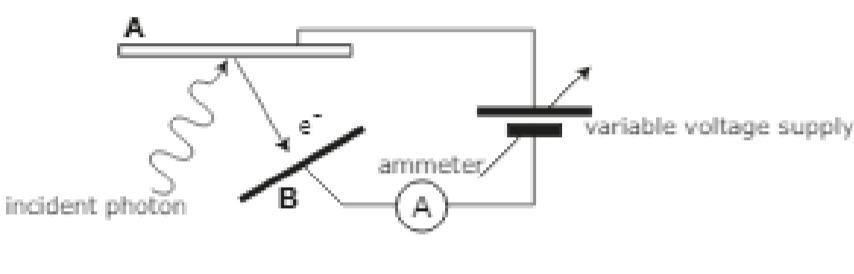
\includegraphics[scale=0.5]{Screenshot (198).png}
        \caption{Schematic of the photoelectric effect set-up \cite{university physics}. The Element denoted A is the Silver Oxide cathode, and the element denoted B is the Nickle anode. The ammeter gives a reading the photo-current due to incident photons and the Variable resister can set a bias voltage over the two plates}
        \label{fig:1}
    \end{figure}
The mercury light source was set a fixed distance from the Photocell tube on an optical bench. The filters were used so that there was only one wavelength of light incident upon the Silver Oxide cathode. The frequency of the photon was found from rearranging equation 1. A bias voltage was
applied to the Nickel anode. The ammeter and current amplifier meant that it was possible to measure when the stopping voltage was met. This was done for 5 different wavelengths so that a graph could be produced of stopping voltage against the frequency of photon causing the photo-current. The experiment was repeated three times for each wavelength of light so that a mean
stopping voltage and standard deviation could be found.
\begin{figure}[ht!]
    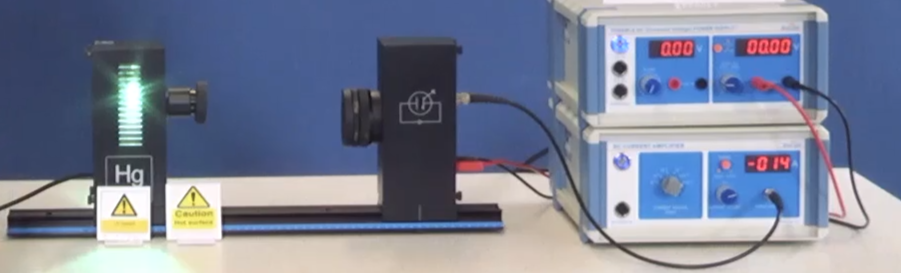
\includegraphics[scale=0.4]{Photocell tube picture.png}
    \caption{A picture showing the apparatus set up. There is an optical bench with a mercury light source and power supply as well as an evacuated photocell tube in a photocell tube holder with aperture control and filters. The photocell tube is connected to a power supply which applied a bias voltage to the nickel anode and an ammeter with current amplifier so that the photo-current could be measured.}
    \label{fig:2}
\end{figure}

\subsection{Improved Methodology}
During this experiment I used a mercury light source to proved the high energy photons to cause the emission of photo-electrons. This light source was able to be capped to stop the incidence of light upon the photocell tube enclosure.\\ 
The photocell tube enclosure used throughout this experiment had aperture control and filters so that the intensity and wavelength of light incident upon the photocell tube could be controlled. The photocell tube used was evacuated of any air to avoid any interference the air may have caused and had a silver oxide cathode and a nickel anode. The photocell tube was able to have a bias voltage applied over it and the photo-current (the current that was a result of the emission of photo-electrons) was able to be measured by an ammeter.\\
The Mercury light source and Photocell tube enclosure were put at a set distance on an optical bench before the experiment commenced
\\
 \begin{figure}[ht!]
    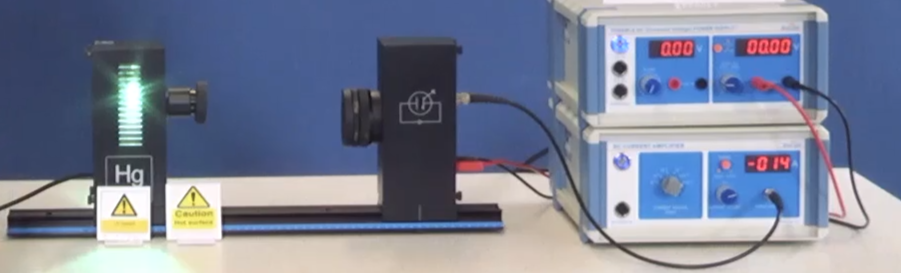
\includegraphics[scale=0.4]{Photocell tube picture.png}
    \caption{A picture showing the apparatus set up. There is an optical bench with a mercury light source and power supply as well as an evacuated photocell tube in a photocell tube holder with aperture control and filters. The photocell tube is connected to a power supply which applied a bias voltage to the nickel anode and an ammeter with current amplifier so that the photo-current could be measured.}
    \label{fig:3}
\end{figure}

During the experiment the Mercury Light source was de-capped and allowed to be incident upon the photocell tube enclosure. The photocell tube enclosure's aperture control was set to the lowest value of 365.4 nanometers. The relation between the frequency and wavelength of electromagnetic radiation means that the frequency of photons making incident upon the silver oxide surface was $\frac{c}{\lambda}$. The high energy light upon the metal surface meant that Photo-electrons were emitted causing a photo-current.\\

Using the ammeter to measure the photo current and a voltmeter to measure the bias voltage applied over the Photocell tube, a bias voltage was increased until there was zero photo-current (which meant that there was no emission of photo-electrons). This Bias Voltage could be used along with the frequency of light to calculate the work function of the silver oxide.
This method was repeated for the remaining 4 filters (which correspond to 4 unique wavelengths) and the results noted so that they could be used for analysis of the phenomenon\\
 \begin{figure}[ht!]
        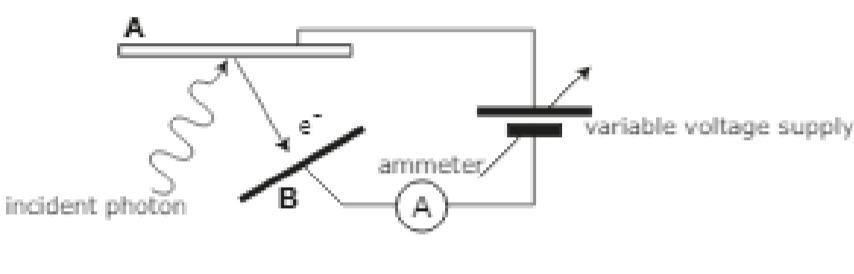
\includegraphics[scale=0.5]{Screenshot (198).png}
        \caption{Schematic of the photoelectric effect set-up \cite{university physics}. The Element denoted A is the Silver Oxide cathode, and the element denoted B is the Nickle anode. The ammeter gives a reading the photo-current due to incident photons and the Variable voltage supply can set a bias voltage over the two plates}
        \label{fig:4}
\end{figure}

\textit{The changes mad to the methodology have improved it as I have tried to go into more detail for each of the steps taken in the experiment to make it easier for someone for follow and understand why these steps are being taken. I have also started with an explanation of the equipment used so that someone could repeat my experiment more easily than before. I have attempted to make the writing style more succinct to make it a nicer read for prospective readers}

























\section{Bibliography}
\begin{thebibliography}{}
   
    \bibitem{1921 Nobel} The Nobel Prize in Physics 1921. NobelPrize.org. Nobel Media AB 2021. Sun. 7 Mar 2021.
   
    \bibitem{Einstein 1905} Einstein A. Über einem die Erzeugung und Verwandlung des Lichtes betreffenden heuristischen Gesichtspunkt. Annalen der physik. 1905;4.
   
    \bibitem{Hertz} Hertz H. Ueber einen Einfluss des ultravioletten Lichtes auf die electrische Entladung. Annalen der Physik. 1887;267(8):983-1000.
   
    \bibitem{statistical mechanics}Landsberg PT. Thermodynamics and statistical mechanics. Courier Corporation; 2014 Mar 5.
   
    \bibitem{Planck}Planck M. Über das gesetz der energieverteilung im normalspektrum. InVon Kirchhoff bis Planck 1978 (pp. 178-191). Vieweg+ Teubner Verlag, Wiesbaden.
   
    \bibitem{university physics} Young H.D, Freedman R.A.University Physics with Modern Physics. Fifteenth Edition.A.L Ford, KZ Estrugo.Uni tied Kingdom:Pearson Education Limited,2020
\end{thebibliography}

    
    


    \end{document}